\documentclass[a4paper,addpoints]{exam}

\usepackage{commath}
\usepackage{siunitx}

% russian integral
\usepackage{scalerel}
\DeclareMathOperator*{\rint}{\scalerel*{\rotatebox{17}{$\!\int\!$}}{\int}}

\qformat{\textbf{\large{Question \thequestion}}\hfill}
\pointsinrightmargin

\begin{document}

\begin{coverpages}

\begin{center}
  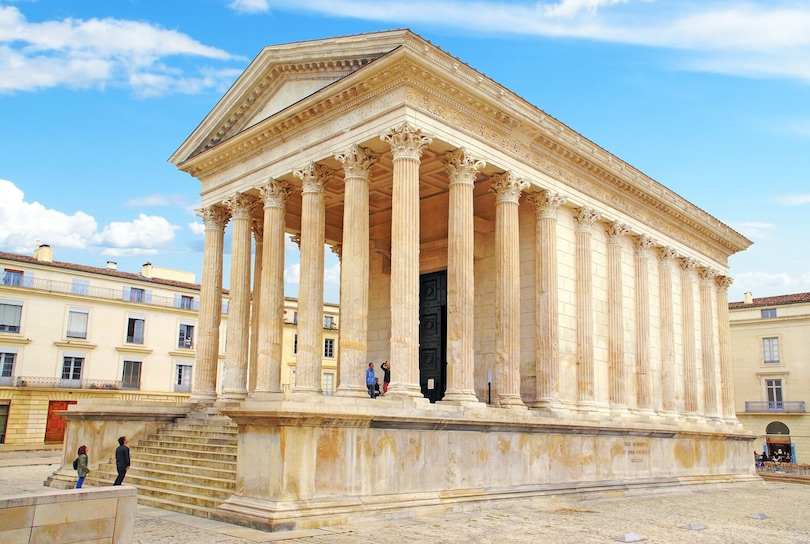
\includegraphics[width=0.6\textwidth]{exam-cover-02}

  \vspace{5mm}

  \textbf{\Huge{Level Three Calculus}}

  \vspace{2mm}

  \textbf{\Huge{Integration}}
\end{center}

\vspace{5mm}

\noindent
\large{There are three questions, worth a total of \numpoints\ marks.\\
       Attempt ALL questions, showing all working.\\
       Read questions carefully before attempting them.\\
       Marks are available for partial answers.\\
       The amount of time expected to be spent per question may not necessarily correlate ``nicely'' to the number of marks.\\
       Diagrams may be used to support answers.\\
       Candidates who do not provide diagrams for some questions may be disadvantaged.\\
       Some marks are given for clarity and neatness of solutions or proofs.}
\vspace{2mm}

\begin{tabular}{ll}
  \textbf{Time Allowed:}& One Hour\\
  \textbf{Achieved:}& 13 marks\\
  \textbf{Merit:}& 22 marks\\
  \textbf{Excellence:}& 31 marks
\end{tabular}

\vfill

\begin{center}
  \gradetable[h][questions]
  \vspace{2mm}

  \textbf{Available Grades:} \textit{Not Achieved}\quad\textit{Achieved}\quad\textit{Merit}\quad\textit{Excellence}
\end{center}

\end{coverpages}

\begin{questions}
  \question
    \begin{parts}
      \part Compute the following indefinite integrals.
        \begin{subparts}
          \subpart[1]
            \begin{displaymath}
              \rint \frac{3t^2 + 2t}{\sqrt{t}} \dif{t}
            \end{displaymath}
          \subpart[1]
            \begin{displaymath}
              \rint 2 \sin 2x \sin (\cos 2x) \dif{x}
            \end{displaymath}
        \end{subparts}
      \part[3] Suppose that the derivative of $ y $ is
            \begin{displaymath}
              \od{y}{x} = \frac{1}{\ln(2) (x + 2)}.
            \end{displaymath}
            If $ y = 3 $ when $ x = 0 $, find $ y $ when $ x = -1 $.
      \part[2] Suppose $ f $ is a continuous function. If $ 0 < x < y < 10 $, $ \rint^{10}_x f(t) \dif{t} = 3 $,  $ \rint^y_0 \dif{t} = 4 $, and
            $ \rint^{x}_{y} f(t) \dif{t} = 2 $, find $ \rint^{10}_0 f(t) \dif{t} $.
      \part[5] The base of a solid is a square with vertices located at $ (1, 0) $, $ (0, 1) $, $ (-1, 0) $, and $ (0, -1) $.
            Each cross-section perpendicular to the $ x$-axis is a semicircle (so the semicircle on the $ x$-axis itself
            has radius 1). Form a definite integral and calculate the volume of the solid.
    \end{parts}

  \question
    \begin{parts}
      \part[2] Compute the following definite integral.
        \begin{displaymath}
          \rint^{\pi/3}_{\pi/4} \csc^2 \theta \dif{\theta}
        \end{displaymath}
      \part[3] Find the area (to 1 decimal place) between the graphs of $ y = \sin x $ and $ y = x^2 - \frac{2(1 + \pi^2)}{\pi} x + \frac{3\pi^2}{4} + 2 $
            shown in in figure \ref{fig:trigintersect}, given that their intersection points are $ (\pi/2, 1) $ and $ (3\pi/2, -1) $.
            \begin{figure}
              \centering
              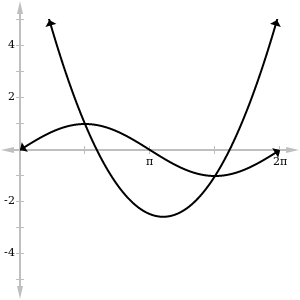
\includegraphics[width=0.35\textwidth]{trigintersect}
              \caption{Two intersecting functions.\label{fig:trigintersect}}
            \end{figure}
      \part The rate of change of a particular animal population over $ t $ days is given by
            \begin{displaymath}
              \od{P}{t} = 1 - \frac{P}{M},
            \end{displaymath}
            where $ M $ is a constant.
        \begin{subparts}
          \subpart[4] Find an explicit formula for $ P $ in terms of $ M $ and $ t $, given that $ P(0) = 100 $.
          \subpart[3] If $ \od{P}{t} = 1 $ when $ t = 0 $, find $ M $. Hence, find the population after 100 days.
        \end{subparts}
    \end{parts}

  \clearpage
  \question
    \begin{parts}
      \part[2] Table \ref{tab:simpsons} gives values of a function $ D(t) $. Use Simpson's rule with $ n = 6 $ to
            approximate $ \rint^{6}_{0} D(t)\dif{t} $.
            \begin{table}
              \centering
              \caption{Data over a network in gigabits per hour, $ D(t) $.\label{tab:simpsons}}
              \begin{tabular}{c|c}
                $ t $ & $ D(t) $\\\hline
                0 & 3.2\\
                1 & 2.7\\
                2 & 1.9\\
                3 & 1.7\\
                4 & 1.3\\
                5 & 1.0\\
                6 & 1.1
              \end{tabular}
            \end{table}
      \part[2] Evaluate the following indefinite integral.
            \begin{displaymath}
              \rint e^x (15 + e^x)^{2017} + 3 \dif{x}
            \end{displaymath}
      \part[4] Suppose $ n $ is an integer constant. If $ y $ is defined implicitly as a function of $ x $ as follows,
            and $ y = 0 $ when $ x = 0 $, find $ y $ when $ x = \frac{1}{n} $.
            \begin{displaymath}
              \od{y}{x} = -(y + 2)(n\pi \sin(x n \pi))
            \end{displaymath}
      \part[4] Using the substitution $ x = \sin \theta $, or otherwise, compute the following indefinite integral.
            \begin{displaymath}
              \rint \frac{1}{\sqrt{1 - x^2}} \dif{x}
            \end{displaymath}
    \end{parts}
\end{questions}
\end{document}
